\documentclass[a4paper]{article}
\usepackage[a4paper, left=15mm, right=15mm, top=10mm, bottom=10mm]{geometry}
\usepackage[utf8]{inputenc}
\usepackage{indentfirst}
\usepackage{amsmath}
\usepackage{amssymb}
\usepackage{graphicx}
\usepackage{float}
\usepackage{amsthm}
\usepackage{hyperref}

\DeclareMathOperator*{\argmin}{arg\,min}

\newcommand{\F}{\mathcal{F}}
\newcommand{\R}{\mathbb{R}}
\newcommand{\conv}{\rm{conv}\,}

\renewcommand{\baselinestretch}{1.3}

\theoremstyle{definition}
\newtheorem{definition}{Notation}[]

\title{CAQM: Convexity Analysis of Quadratic Maps}
\date{}
\author{Anatoly Dymarsky, Elena Gryazina, Boris Polyak, Sergei Volodin}

\begin{document}
\maketitle
MatLab library CAQM is a tool to analyze geometric properties of quadratic maps (manifolds of real-valued solutions of systems of quadratic equations).
Main functionality described below is contained in 5 MatLab functions located in the main folder.
Additional functionality is described in the accompanying file {\tt library.pdf}.

\section*{Installation and Testing}
The library does not require additional installation beyond unpacking and adding the main folder, including subfolders, to the Matlab path.
To test installation and functionality one can run {\tt CAQMtest.m} located in {\tt tests} folder.
A sucessful run should end with {\tt TEST PASSED} message.
Full output and other details can be found in this \href{https://youtu.be/Ikh_GDHnu-4}{video}.

\section*{Notations}
\begin{enumerate}
\item Real case, the map $f\colon \mathbb{R}^n\to\mathbb{R}^m$
\begin{equation}
f_k(x)=x^TA_k x+2b_k^Tx ,\quad A_k=A_k^T ,\quad x, b_k\in \mathbb{R}^n ,\quad i=k\dots m . \label{real}
\end{equation}
\item Complex case, the map $f\colon \mathbb{C}^n\to\mathbb{R}^m$
\begin{equation}
f_k(x)=x^*A_k x+b_i^*x+x^*b_k ,\quad A_k=A_k^* ,\quad x, b_k\in \mathbb{C}^n ,\quad i=k\dots m ,\label{complex}
\end{equation}
where $\cdot^*$ is Hermitian conjugate.
\end{enumerate}

We will use $\mathbb{V}$ to denote $\mathbb{R}^n$ in the real case and $\mathbb{C}^n$ in the  complex case.
We also use the following notations:\\

\theoremstyle{definition}
\begin{definition}
For a vector $c=(c_1,...,c_m)$ and a tuple of vectors $b=(b_1,...,b_m), \ b_k \in \mathbb{V}$, or a tuple of $n\times n$ matrices $A=(A_1,...,A_m), \  A_k\in \mathbb{V}^2$, the dot product is defined as follows,
\begin{eqnarray}
c\cdot b=\sum\limits_{k=1}^m c_k\, b_k ,\qquad
c\cdot A=\sum\limits_{k=1}^m c_k\, A_k\ . \nonumber
\end{eqnarray}
\end{definition}

\begin{definition}
The image of $f$ is denoted as $F$,
	$$F=f(\mathbb{V})\subset \mathbb{R}^m\ .$$
\end{definition}
\begin{definition} The convex hull of $F$ is denoted as $G$:
	$$G=\conv (F)\subset \mathbb{R}^m\ .$$
\end{definition}
\begin{definition} The boundary points of $F$ touched by a supporting hyperplane with the normal vector $c\in\mathbb{R}^m$,
	$$\partial F_c=\argmin\limits_{y\in F}(c\cdot y)$$
\end{definition}
\begin{definition} The boundary points of $G$ touched by a supporting hyperplane with the normal vector $c\in\mathbb{R}^m$,
	$$\partial G_c=\argmin\limits_{y\in G}(c\cdot y)$$
\end{definition}
\begin{definition}\label{ex:c_minus}
	Set of normal vectors $c$, such that $\partial F_c$ is nonconvex is denoted as $C_-$,
	$$
	C_-=\{c\in\R^m\,\big|\,\mbox{Set }\partial F_c\mbox{ is nonconvex}\}
	$$
\end{definition}

\section*{Functionality}
The library consists of several functions, each of them is defined in a separate .m file.
Input format for specify the quadratic map is as follows.

\begin{itemize}
\item The array $A(i, j, k)$ denotes $i$'th row and $j$'th column of a $n\times n$ matrix $A_k\in\mathbb{V}^2$
\item The array $b(i, k)$ denotes $i$'th element of a vector $b_k\in\mathbb{V}$
\end{itemize}

\begin{enumerate}
\item {\bf Feasibility membership oracle\ \ \  }{\tt \large  infeasibility$\_$oracle.m}
\begin{verbatim}
is_infeasible = infeasibility_oracle(A, b, y)
\end{verbatim}
{\it Input:}
\begin{itemize}
\item the map $f$ specified by matrices $A_k$ and vectors $b_k$,
\item point $y\in\mathbb{R}^m$.
\end{itemize}
{\it Output:} determines if $y\in G$, returns {\tt is\_infeasible}=1 if $y\notin G$, {\tt is\_infeasible}=0 if $y\in G$.

\begin{figure}[H]
	\centering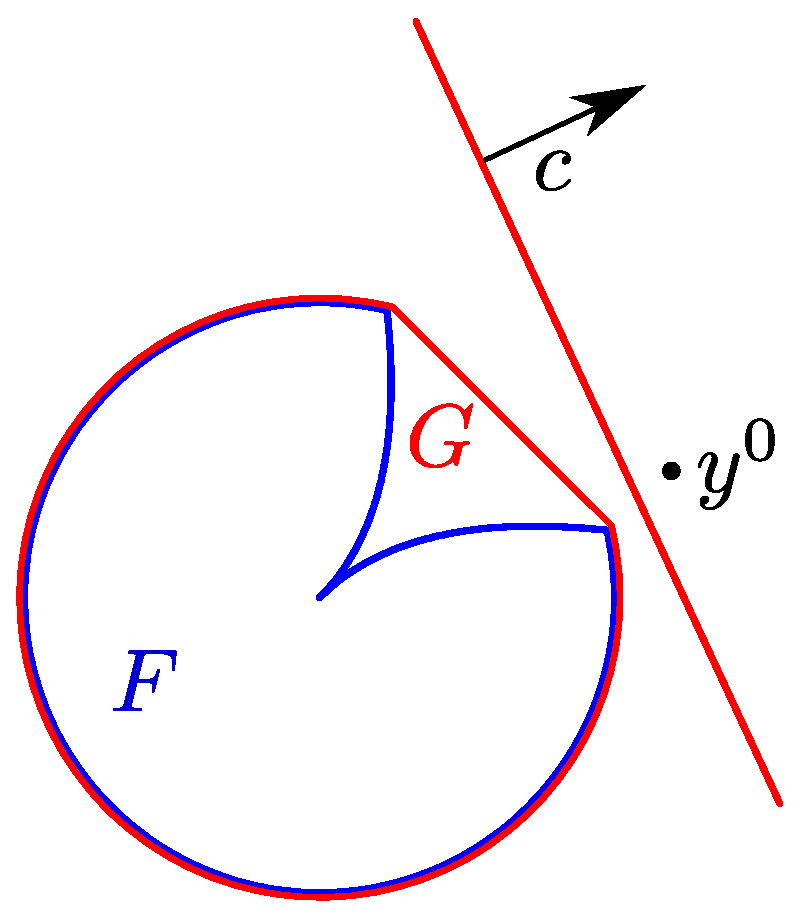
\includegraphics[width=100pt]{fig/infeasibility_oracle}
	\caption{Infeasibility oracle: hyperplane orthogonal to $c$ separates the point $y$ from the convex hull $G$ of $F$}
\label{fig:one}
\end{figure}

This function attempts to certify that the point $y$ does not belong to the convex hull $G$ of $F$ by separating $y$ and $G$ by an appropriate hyperplane. This is illustrated in Fig.~\ref{fig:one}, see Theorem 3.2 in the accompanying article for details.
The function returns {\tt is\_infeasible}$=1$ if the desired hyperplane was found. In this case $y\notin G$ and consequently $y\notin F$, implying there is no $x\in \mathbb{V}$ such that $y=f(x)$, i.e.~this point is infeasible. If the hyperplane was not found the function returns {\tt is\_infeasible}$=0$, which means the feasibility  of $y$ with respect to $F$ is uncertain. We note that feasibility of $y$  is exactly the same as solvability of the system of quadratic equations $y=f(x)$ with real-valued $x$ when the map $f$ is real, or with $x$ and $x^*$ being complex conjugate to each other if $f$ is complex as defined in eq.~\eqref{complex}.

\item {\bf Boundary oracle\ \ \  }{\tt \large boundary$\_$oracle.m}
\begin{verbatim}
[t, is_in_F] = boundary_oracle(A, b, y, d)
\end{verbatim}
{\it Input:}
\begin{itemize}
	\item the map $f$ specified by matrices $A_k$ and vectors $b_k$,
	\item a point $y\in G$,
	\item a direction $d\in\R^m$.
\end{itemize}
{\it Output:}  finds and returns distance $t$ to the boundary of $G$ from the point $y$ inside $G$ in the direction $d$; verifies if boundary point belongs to $F$. 


\begin{figure}[H]
	\centering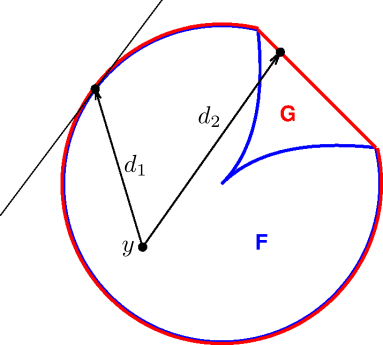
\includegraphics[width=100pt]{fig/boundary_oracle}
	\caption{Boundary oracle: distance from $y$ to the boundary $\partial G$ in the direction $d$. The boundary point of $G$ may or may not belong to $\partial F$ (cases of $d=d_1$ and $d=d_2$ respectively).}
\label{fig:two}
\end{figure}


This function finds point $y+t\,d$ on the boundary $\partial G$ with the largest $ {t} = \sup\{\tau\big| y+\tau d\in G\}$ and checks if this point belongs to $F$. 
This is illustrated in Fig.~\ref{fig:two}, see Theorem ??!! in the accompanying article for details. The function returns $\tt t$ with the value of $t$, variable
	{\tt  is\_in\_F}$=1$ if the boundary point $y+t\,d$ belongs to $F$, and variable {\tt  is\_in\_F}$=0$ if feasibility of $y+t\,d$ with respect to $F$ is uncertain.\\
{\it Exception:}  if on input $y\notin G$ or $\partial G$ is not smooth at the boundary point $y+t\,d\in \partial G$ the function produces an exception. 



%\item {\bf Normal vector at the boundary\ \ \  }{\tt get\_c\_from\_d.m} 
%\begin{verbatim}
%c = get_c_from_d(A, b, y, d)
%\end{verbatim}
%{\it Input:}
%\begin{itemize}
%	\item the map $f$ specified by matrices $A_k$ and vectors $b_k$,
%	\item a point $y\in G$,
%	\item a direction $d\in\R^m$.
%\end{itemize}
%{\it Output:}  finds point $y+t\,d$ at the boundary of $G$ and returns vector $c$ normal to $\partial G$ at that point 
%
%
%\begin{figure}[H]
%	\centering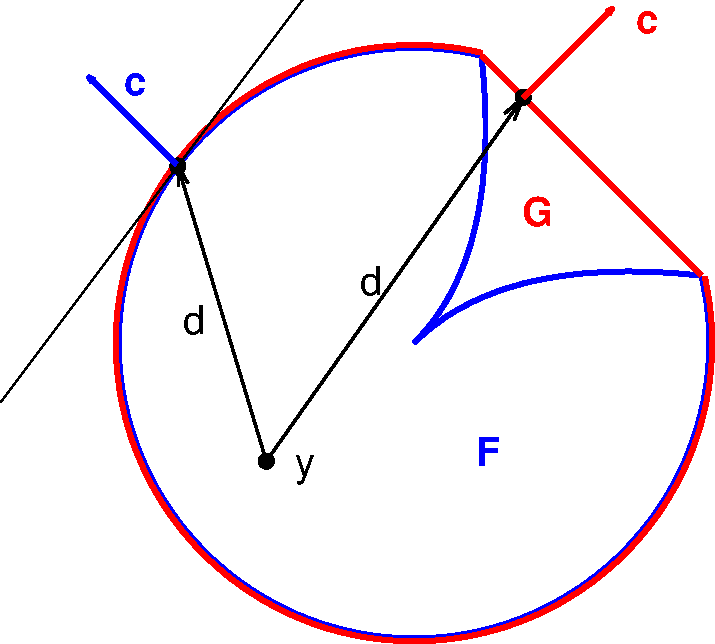
\includegraphics[width=100pt]{fig/get_c_from_d}
%	\caption{Normal vector at the boundary: vector $c$ normal to $\partial G$ at the boundary point $y+td$. This function only ``knows" about $G$ and does not distinguish between points $y+td$ which do and do not belong to $F$.}
%\label{fig:three}
%\end{figure}
%
%This function finds boundary point $y+td\in \partial G$ and calculates vector $c$ normal to $\partial G$ at that point by using the dual formulation of the optimization problem, see ?? of the accompanying article. This is schematically illustrated in Fig.~\ref{fig:three}. The function returns vector variable $\tt c$ with the value of $c$ .
%
%{\it Exception:} if on the input $y\notin G$ or the normal vector to $\partial G$ at $y+td$ does not exist (because $\partial G$ is not smooth at this point)  the function produces an exception. 

\item {\bf ``Non-convex direction"\ \ \  }{\tt get\_c\_minus.m} 
	\begin{verbatim}
	c = get_c_minus(A, b, [y], [k])
	\end{verbatim}
{\it Input:}
\begin{itemize}
	\item the map $f$ specified by matrices $A_k$ and vectors $b_k$,
	\item  $[$optional$]$ a point $y\in G$,
	\item $[$optional$]$ number of iterations $k$.
\end{itemize}
{\it Output:}  finds and returns vector $c$ such that $\partial F_c$ is nonconvex through a stochastic algorithm using up to $k$ iterations; returns empty vector if such $c$ was not  found.\\
{\it Exception:} really??!!
%\\[-1pt]

	This function consequently generates up to $k$ random directions $d$ and for each one finds vector $c$ normal to $\partial G$ at the boundary point $y+t\, d\in \partial G$.  Next it finds $\partial_c F$, the intersection of $F$ with the supporting hyperplane orthogonal to $c$ and checks if it is nonconvex.  We note that non-convexity of $\partial_c F$ implies non-convexity of $F$. This function stops and returns $c$ if non-convexity of $\partial_c F$ was established during one of the iterations, and empty vector ${\tt c=[\ ]}$ otherwise. 
If $y$ and $k$ are not specified, the function uses default values $y=f(0)=0$ and $k=10$.


\item {\bf Nonconvexity certificate\ \ \  }{\tt nonconvexity\_certificate.m} 
	\begin{verbatim}
	is_nonconvex = nonconvexity_certificate(A, b, [y], [k])
	\end{verbatim}
{\it Input:}
\begin{itemize}
	\item the map $f$ specified by matrices $A_k$ and vectors $b_k$,
	\item  $[$optional$]$ a point $y\in G$,
	\item $[$optional$]$ number of iterations $k$.
\end{itemize}
{\it Output:} attempts to establish if $F$ is convex, returns {\tt is\_nonconvex}=$1$ if $F$ is non-convex,  {\tt is\_nonconvex}=$0$ if uncertain.

	
	This function calls {\tt get\_c\_minus} and returns  {\tt is\_nonconvex}=$1$ if the latter returns a non-trivial $c$. 


\item {\bf Positive-definite $c\cdot A$\ \ \ }{\tt get\_c\_plus.m}
\begin{verbatim}
	c_plus = get_c_plus(A, k)
\end{verbatim}

{\it Input:}
\begin{itemize}
	\item matrices $A_k$
	\item $[$optional$]$ number of iterations $k$
\end{itemize}
{\it Output:} finds and returns vector $c_+$ such that $c_+\cdot A\succ 0$.\\
{\it Exception:} if $c_+$  was not found during $k$ random iterations.

	
	This function generates a random ``seed" which is used to find $c_+$ such that $c_+\cdot A\succ 0$. If successful, the function terminates and returns $c_+$ on the exit, otherwise the search attempt is repeated up to $k$ times. If not specified explicitly, the default value of $k=10$. If $c_+$ is not found during $k$ iterations the function produces an exception. 
	
\item {\bf Convex subpart\ \ \ }{\tt get\_z\_max.m}
\begin{verbatim}
z_max = get_z_max(A, b, c_plus, [z_max_guess], [k])
\end{verbatim}
{\it Input:}
\begin{itemize}
	\item the map $f$ specified by matrices $A_k$ and vectors $b_k$,
	\item vector $c_+$ such that $c_+\cdot A\succeq 0$,
	\item $[$optional$]$ the guess value  $z^{\rm guess}_{\rm max}$,
	\item $[$optional$]$ number of iterations $k$.
\end{itemize}
{\it Output:} finds and returns maximal value $z_{\max}$ such that the compact part of $F$ ``cut" by the hyperplane  $c_+ \cdot (y-y_0)=z_{\max}$, where $y_0\in \partial_{c_+}F$, is still convex. \\
{\it Exception:} produces an exception if non-convexity of $F$ confined within the half-plane $c_+ \cdot (y-y_0)\leq z^{\rm guess}_{\rm max}$  has not been established.  ??!!

\begin{figure}[H]
	\centering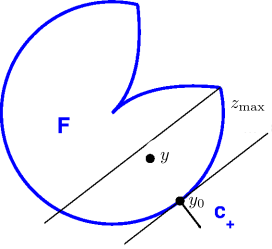
\includegraphics[width=100pt]{fig/get_z_max}
	\caption{Maximal value of $z_{\max}$ such that  the subpart of $F$, $F_{z_{\rm max}}\equiv \{y\, | y\in F, c_+ \cdot (y-y_0)\leq z_{\rm max}\}$, which is ``cut" from $F$ by a hyperplane orthogonal  to $c_+$ is still convex.}
\label{fig:four}
\end{figure}



This function returns maximal value $z_{\max}$ such that the hyperplane perpendicular to $c_+$ and located distance $z_{\max}$ away from the boundary of $F$ is still convex. More precisely,  the compact part of $F$ confined by the half-space $\{y\, |c_+ \cdot (y-y_0)\leq z^{\rm guess}_{\rm max}\}$ is convex. Here $y_0\in \partial_{c_+}F$, and since $c_+\cdot A\succ 0$, the set $\partial_{c_+}F$ consists of only one point $y_0$. The geometric meaning of $z_{\max}$ is illustrated in Fig.~{fig:four}. 
The function first tries to identify ``non-convex directions" $c_-$ using {\tt get\_c\_minus} and then ``follow" each non-convexity to the smallest value of $z$. This is described in detail in the section ??!! of the accompanying paper.
If no ``non-convex directions" found, the function returns $z^{\rm guess}_{\rm max}$ assuming the part of $F$ confined within the half-space $\{y\, |c_+ \cdot (y-y_0)\leq z^{\rm guess}_{\rm max}\}$ is convex. 
In case the input value of $c_+$ does not satisfy $c_+\cdot A\succ 0$, the function produced as exception ???
If the maximal number of iterations $k$ (to be used with {\tt get\_c\_minus}) is not specified on input, the default value $k=10$ (or $k=100$?) is used by default. The guess value $z^{\rm guess}_{\rm max}$ is supposed to be substantially large to detect non-convexity of $F$. If it is not specified on input, a default value of $z^{\rm guess}_{\rm max}=10 {\rm Tr}(c_+\cdot A)$ is used.  It is important to keep in mind that the algorithm is heuristic. A non-trivial return value $z_{\max}\neq z^{\rm guess}_{\rm max}$ does not guarantee convexity of  $F_{z_{\rm max}}\equiv \{y\, | y\in F, c_+ \cdot (y-y_0)\leq z_{\rm max}\}$, but only that $\{y\, | y\in F,c_+ \cdot (y-y_0)\leq z\}$ for any $z>z_{\rm max}$ is non-convex. Nevertheless, increasing $k$ would increase certainty (in the probabilistic sense) that $F_{z_{\rm max}}$ is indeed convex. 

\end{enumerate}
\end{document}
